\subsection{V-Model}\label{chapter_V_MODEL}

The project was realized on the basis of the V-Model. The V-Model is a common graphical model to plan an engineering process, that get's customized for each project. In the following, the customized V-Model for this project will be explained.

\begin{figure}[htbp]
	\centering
		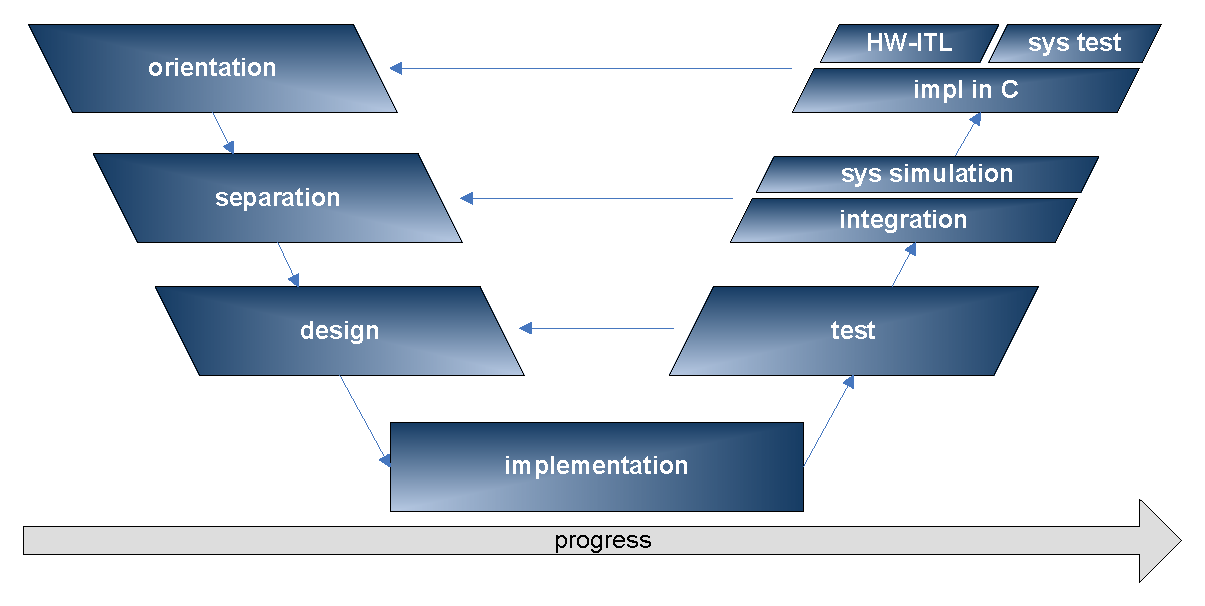
\includegraphics[width=1.00\textwidth]{03_Grafiken/V_Model.pdf}
	\caption{Customized V-Model for this project}
	\label{fig:V_Model}
\end{figure}

Due to a solid basis, on which this project can be build on, the first thing to do is to learn the ropes. The main topic in this step is to understand the quadrocopter's physical model and its already existing model in MATLAB Simulink - and certainly the functionality of a state space controller. An other topic of the orientation-part is to define the requirements. \\
The next step is to separate the relevant part of the Simulink model, so it is possible to work at one 'module', which alleviates to keep the overview. On the basis of this separate part, the next step can be done, which is the beginning of the real project - the design of the state space controller. The lowermost crossbar is the main topic in this engineering process, which means the implementation of the state space controller in MATLAB Simulink. \\
The lowermost part of the right leg of the 'V' includes the test, in this case the simulation, of the implemented state space controller. If there are failures - for example unexpected behavior of a controlled variable, the way follows the lowermost arrow, which guides from the right to the left, back to the design of the state space controller. This circle gets run through, until there are no failures at all. Then the process climbs to the next step, in this case the integration of the state space controller into the original, non-separated Simulink model of the quadrocopter. Then testing, which means still simulation, starts again. If there are failures, the way follows the middle horizontal arrow back to the separation part, because apparently the separated process and the original process don't match. If there are no failures in the system-simulation-part, the next step upward to 'implementation in C' can be done. In this part the graphical model of Simulink gets converted in C-code which is executable by the microcontroller installed in the quadrocopter. This code has to be tested \textbf{H}ardware-\textbf{I}n-the-\textbf{L}oop (HIL) on the real microcontroller. This means, that the code is executed on the real microcontroller, but the output, in this case the actuating variables, gets looped back into the simulation in MATLAB Simulink, which safes ressources, because critical failures can be detected without risking a crash of the quadrocopter. Last but not least, if everything looks great in the HIL simulation, the state space controller gets tested and fine-tuned 'on the fly' with the quadrocopter.

This document leads through this whole engineering process chapter by chapter, starting with understanding the quadrocopter's physical model (chapter \ref{chapter_PHYSICAL_MODEL}) and its model in MATLAB Simulink (chapter \ref{chapter_MATLAB_MODEL}). The next step is to understand the background and layout of a state space controller in chapter \ref{chapter_THEORY}. Then, with this knowledge, the next step is to design and implement the controller in MATLAB/Simulink in chapter \ref{chapter_DESIGN_AND_IMPL} and run simulations in MATLAB Simulink to validate the functionality of the controller in chapter \ref{chapter_TEST}. After that, the implementation of the controller in C is the topic of chapter \ref{chapter_IMPLC}, leading to the HIL tests, just as the tests with the real copter in chapter \ref{chapter_TEST}.
At the end of this document you can find some future prospects in chapter \ref{chapter_FUTUREPROSPECTS}.

With the next chapter this documentation changes over to the engineering process, starting with the physics of the quadrocopter, the first step in the V-Model.